\documentclass{beamer}
\usetheme{Copenhagen}
\usecolortheme{beaver}
\usefonttheme{structurebold}
\usepackage{multirow}
\usepackage{hyperref}
\title{Body Fat Prediction}
\author{Chao Chang, Yezhou Li, Shuyang Chen, Ping Yu}
\institute{University of Wisconsin Madison}
\date{October 10, 2019}


\begin{document}
\begin{frame}
\titlepage
\end{frame}


\frame{
\frametitle{Background and Goal}
\begin{itemize}
\item An accurate measurement of body fat is costly and it is desirable to have easy methods of estimating body fat that are convenient. 
\item Come up with a simple, robust and precise model with \textbf{two} body measurements to calculate body fat.
\end{itemize}
}

\frame{
\frametitle{Data Cleaning: Examine Outliers}
\begin{columns}

  \column{0.6\textwidth}
  \begin{itemize}
  \item   The $216th$ example 
    \begin{itemize}
      \item He has the largest body fat of 45.1\% and his density is 0.995.
      \item Delete this point.
    \end{itemize}
   \vskip 0.5cm
   \item The $182nd$ example
    \begin{itemize}
        \item He has a body fat of 0.
        \item His body fat is $-3.16$ computed by the bodyfat-density formula, which is impossible.
        \item Delete this point.
    \end{itemize}
  \end{itemize}
  
  \column{0.4\textwidth}
      \begin{figure}
      \centering
      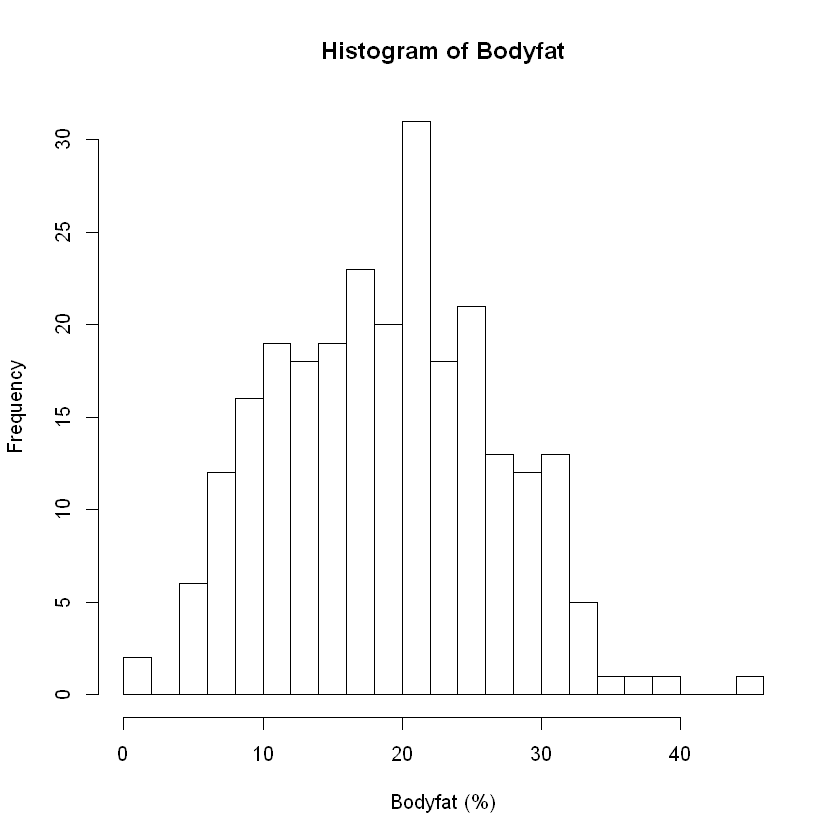
\includegraphics[scale=0.17]{bodyfat}
      \caption{Histogram of body fat}
      \end{figure}
      
  \end{columns}
} 

\frame{
\frametitle{Data Cleaning: Examine Outliers}
\begin{columns}

  \column{0.5\textwidth}
  \begin{itemize}
  \item   The $42nd$ example has the shortest height of 29 inches but his other measurements are normal
\item Impute his height using ADIPOSITY (BMI) formula. $\Rightarrow 69.4$ inches.
\item Keep this point.
  \end{itemize}
  
  \column{0.5\textwidth}
      \begin{figure}
      \centering
      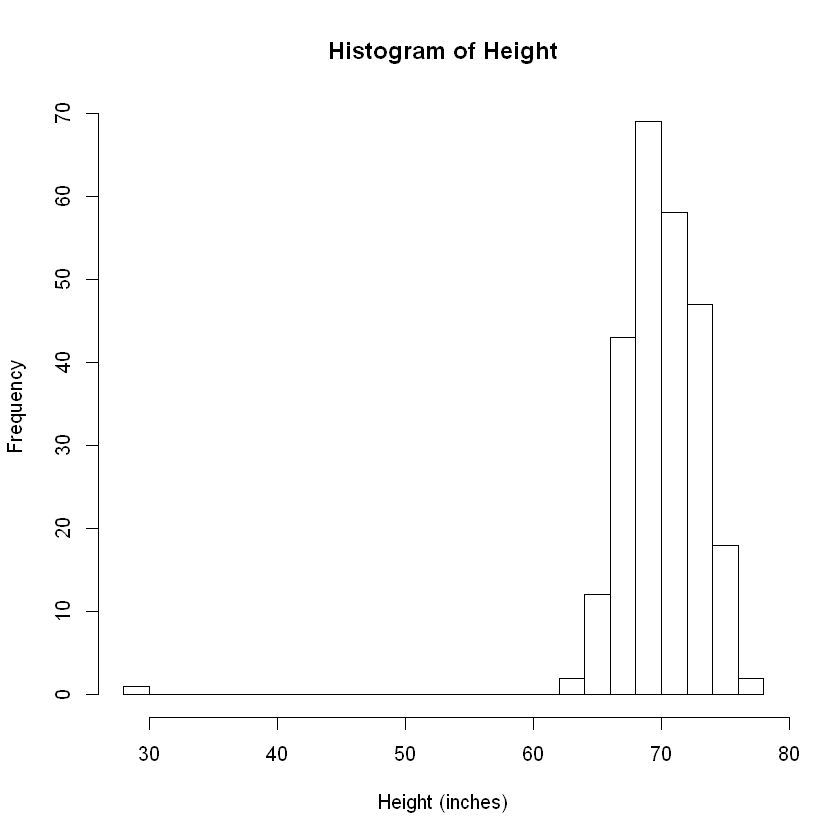
\includegraphics[scale=0.2]{height}
      \caption{Histogram of height}
      \end{figure}
      
  \end{columns}
} 


\frame{
\frametitle{Data Cleaning: Examine Outliers}
\begin{columns}

  \column{0.5\textwidth}
  \begin{itemize}
\item The $39th$ man is the fattest person with the largest weight, abdomen, chest, hip, thigh, knee, biceps, wrist and adiposity.
\item Keep this point.
  \end{itemize}
  
  \column{0.5\textwidth}
      \begin{figure}
      \centering
      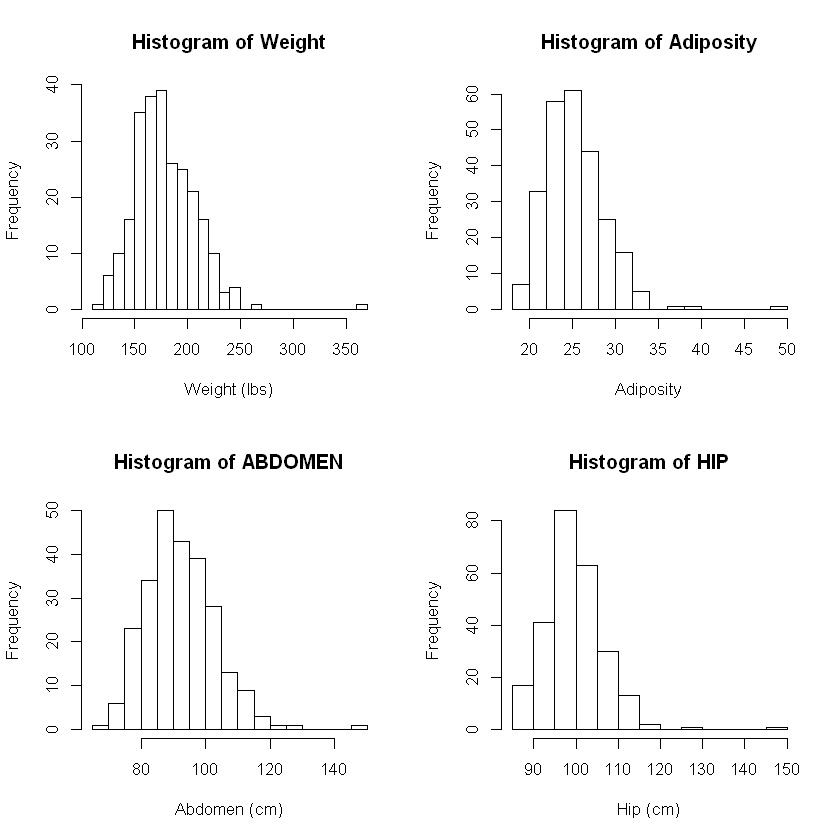
\includegraphics[scale=0.2]{weight}
      \caption{Histogram of weight, adiposity, abdomen and hip}
      \end{figure}
      
  \end{columns}
}

\frame{
\frametitle{Data Cleaning: Examine Outliers}
We compute the \textbf{ADIPOSITY (BMI)} using weight and height to see whether there are some wrong records in this variable:
\begin{table}[]
    \centering
    \begin{tabular}{c|c}
        \hline
         ID & Difference  \\
         \hline
         163 & 3.007 \\
         221 & 2.822 \\
         156 & 0.306 \\
         235 & 0.242 \\
         116 & 0.236 \\
         86 & 0.230 \\
         \hline
    \end{tabular}
    \caption{Difference between records and computed value of Adiposity}
    \label{tab:my_label}
\end{table}

\begin{itemize}
    \item The $163rd$ and $221st$ examples' difference are much larger than others. 
    \item Delete these two points.
\end{itemize}
}


\frame{
\frametitle{Data Cleaning: Final Data Set}
\begin{itemize}
\item Delete $163rd, 182nd, 216th, 221st$ examples.
\item The final data set has $248$ examples and $14$ variables.
\end{itemize}

}

\frame{
\frametitle{Models}
\begin{itemize}
\item Linear model:
    $$Bodyfat_i = \alpha_0 + \alpha_1 ABDOMEN_i + \alpha_2 WRIST_i + \epsilon_i, \epsilon_i \sim N(0, \sigma_1^2)$$
\item Fraction model:
    $$Bodyfat_i = \frac{\beta_1 ABDOMEN_i + \beta_2}{WEIGHT_i} + \gamma_i, \gamma_i \sim N(0, \sigma_2^2)$$
\end{itemize}
}


\frame{
\frametitle{Linear Model: Variable Selection}
\begin{itemize}
  \item Stepwise variable selection
  \item Criterion: BIC
  \begin{itemize}
      \item Models selected by AIC have too many variables.
      \item Using BIC, both forward and backward selection give us a model with four variables:
      $$Bodyfat \sim Weight + Abdomen + Forearm + Wrist$$
  \end{itemize}
\end{itemize}
}

\frame{
\frametitle{Linear Model: Collinearity Problem}
The VIF values of four predictors:
\begin{table}
\begin{tabular}{l | c c c c }
\hline
Predictor & Weight & Abdomen & Forearm & Wrist \\
\hline 
VIF & 7.70 & 5.51 & 1.70 & 2.12 \\ 
\hline
\end{tabular}
\caption{VIF of four predictors}
\end{table}



\begin{itemize}
\item \textbf{Weight} has some collinearity problem.
\item Drop weight to see whether the model performance changes a lot.
\end{itemize}
}

\frame{
\frametitle{Linear Model: Final model}
Divide the full data set into training ($70\%$) and test set ($30\%$).
    \begin{table}[]
    \centering
    \begin{tabular}{l|ccc}
        \hline
         Models & RMSE & $R^2$ \\
         \hline
         Four variables & 4.17 & 0.71 \\
         Abdomen + Forearm + Wrist & 4.33 & 0.69 \\
         \textbf{Forearm + Wrist} & \textbf{7.08} & \textbf{0.17} \\
         Abdomen + Wrist & 4.33 & 0.69 \\
         Abdomen + Forearm & 4.34 & 0.68 \\
         Weight + Abdomen & 4.27 & 0.70 \\
         \hline
    \end{tabular}
    \caption{Model performance}
\end{table}

\begin{itemize}
    \item The best linear model (using the full data set) is:
    $$\text{Bodyfat} = 0.682 \times \text{Abeomen} -2.022 \times \text{Wrist} - 7.256, R^2 = 0.6832$$
\end{itemize}
}

\frame{
\frametitle{Fraction Model: Logics}
\begin{itemize}
    \item There is a linear relationship between body fat and $\frac{1}{Density}$.
        $$Bodyfat = \frac{495}{Density} - 450$$
    \item By physics theorem:
        $$\frac{1}{Density} = \frac{Volume}{Weight}$$
    \item We already have accurate measurement of weight and we try to build a linear model to estimate volume.
    \item Restricted by the number of predictors we can use ($2$), the model we try to construct is:
        $$Bodyfat_i \sim \frac{\beta_1 X_i + \beta_2}{Weight_i} + \beta_3$$
\end{itemize}
}


\frame{
\frametitle{Fraction Model: Variable Selection}
Use the 10-fold cross validation, we iterate through all $14$ variables.
\begin{columns}

  \column{0.5\textwidth}
  \begin{itemize}
      \item No mater we sort by RMSE or the $R^2$, \textbf{Abdomen} stands out among all of the variables.
  \end{itemize}
  
  \column{0.5\textwidth}
  \begin{table}[]
      \centering
      
      \begin{tabular}{l|cc}
           \hline
           Varible & RMSE & $R^2$ \\
           \hline
          \textbf{ABDOMEN} & \textbf{4.06} & \textbf{0.72} \\ 
          ADIPOSITY & 5.10 & 0.55 \\ 
          CHEST & 5.41 & 0.51 \\ 
          AGE & 5.51 & 0.47 \\ 
          WRIST & 5.73 & 0.43 \\ 
          HEIGHT & 5.75 & 0.51 \\ 
          HIP & 5.76 & 0.43 \\ 
          THIGH & 5.84 & 0.40 \\ 
          NECK & 5.87 & 0.41 \\ 
          ANKLE & 5.88 & 0.41 \\ 
          KNEE & 5.90 & 0.40 \\ 
          FOREARM & 5.92 & 0.39 \\ 
          BICEPS & 5.92 & 0.39 \\ 
           \hline
      \end{tabular}
      \caption{Model performance}
  \end{table}
  \end{columns}
}

\frame{
\frametitle{Fraction Model}
After we fit the model using the full data, the result is the following with $R^2=0.7089$:
\begin{table}[]
    \centering
    \begin{tabular}{l|cccc}
        \hline
         & Estimate & Std. Error & p value  \\
         \hline
         Intercept & -2.515 & 3.559 & 0.48 \\
         invWeight & -10736.297 & 438.877 & $<2e-16^{***}$ \\
         ABD-WEI & 158.986 & 9.566 & $<2e-16^{***}$ \\
         \hline
    \end{tabular}
\end{table}
The intercept is not significant so we try to drop the intercept. The model without the intercept has $R^2=0.9605$.
\begin{table}[]
    \centering
    \begin{tabular}{l|cccc}
        \hline
         & Estimate & Std. Error & p value  \\
         \hline
         invWeight & -10632.653 & 413.229 & $<2e-16^{***}$ \\
         ABD-WEI & 153.050 & 4.573 & $<2e-16^{***}$ \\
         \hline
    \end{tabular}
\end{table}
}


\frame{
\frametitle{Fraction Model: Final Model}
The best fraction model is:
$$Bodyfat_i = \frac{153.05\text{Abdomen}_i - 10632.653}{\text{Weight}_i}, R^2=0.9605$$
}


\frame{
\frametitle{Final Model}
\begin{table}[]
\begin{tabular}{l|ll|ll}
\hline
               & \multicolumn{2}{c|}{RMSE}                                    & \multicolumn{2}{c}{$R^2$}                    \\ \hline
Model          & \multicolumn{1}{c}{10-fold} & \multicolumn{1}{c|}{full data} & \multicolumn{1}{c}{10-fold} & \multicolumn{1}{c}{full data} \\ \hline
Linear model   & 4.20                        & 4.207                          & 0.702                       & 0.6832                        \\
Fraction model & 4.03                        & 4.036                          & 0.723                       & 0.9605                        \\ \hline
\end{tabular}
\caption{Comparison between linear and fraction model}
\end{table}
The final model is:
$$Bodyfat_i = \frac{153.05\text{Abdomen}_i - 10632.653}{\text{Weight}_i}$$
}

\frame{
\frametitle{Model Diagnose}
\begin{figure}
      \centering
      \includegraphics[scale=0.5]{dig}
      \caption{Diagnose plots of fraction model}
      \end{figure}
}

\frame{
\frametitle{Our Rule of Thumb}
\begin{block}{Rule of thumb}
$$\text{Bodyfat}_i = \frac{153\times \text{Abdomen}_i - 1.06\times 10^4}{\text{Weight}_i}$$
\end{block}

\textbf{Interpretation}: $153$ times the ratio between abdomen and weight, and then minus $1.06\times10^4$ times the inverse of weight.
}

\frame{
\frametitle{Shinny Application}
Our shinny application URL is: \url{https://clarefrost.shinyapps.io/shiny_628_group4/}
}

\frame{
\frametitle{}
\begin{center}
\textbf{  Thank You}
\end{center}
}
\end{document}